\chapter{Literature Review}
\label{ch:background}

\section{A History of DeepFakes}

% \begin{itemize}
%     \item More detailed explanation of deepfakes
%     \item How are they generated
%     \begin{itemize}
%         \item GANs
%         \item assorted other AI shenanigans
%     \end{itemize}
% \end{itemize}

\subsection{Photo Manipulation}

Humans have been manipulating photographs since the 1860s when a composite of United States President Abraham Lincoln was composited onto fellow politician John Calhoun's body\cite{singh2018art} as shown in Figure \ref{fig:lincoln}. Photo tampering was then used throughout history as a way to shape opinions and beliefs of individuals by altering supposed ``evidence". As photography was still an entirely analogue process, editing a photo was significantly harder than it is today but nevertheless it still was done when deemed necessary. Another famous example is the removal of Nikolai Yezhov in 1940 from a 1937 photo (Figure \ref{fig:stalin-yezhov}) with Joseph Stalin after the ``Great Purge" in the Union of Soviet Socialist Republics.

\begin{figure}[H]
    \centering
    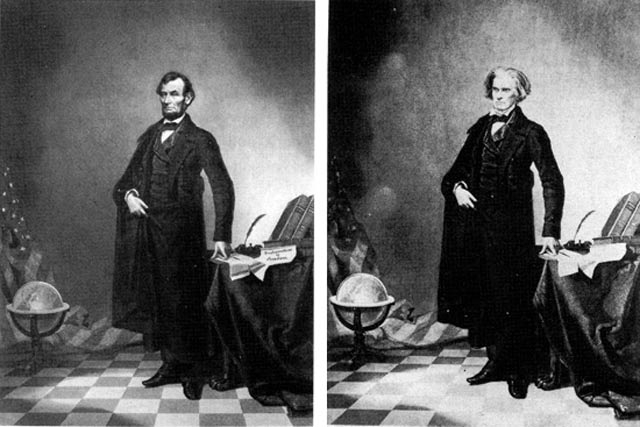
\includegraphics[width=0.5\linewidth]{dissertation//figures/lincoln1960.jpg}
    \caption{A spliced portrait of Abraham Lincoln (left) with the original (right)\cite{singh2018art}}
    \label{fig:lincoln}
\end{figure}

\begin{figure}[H]
    \centering
    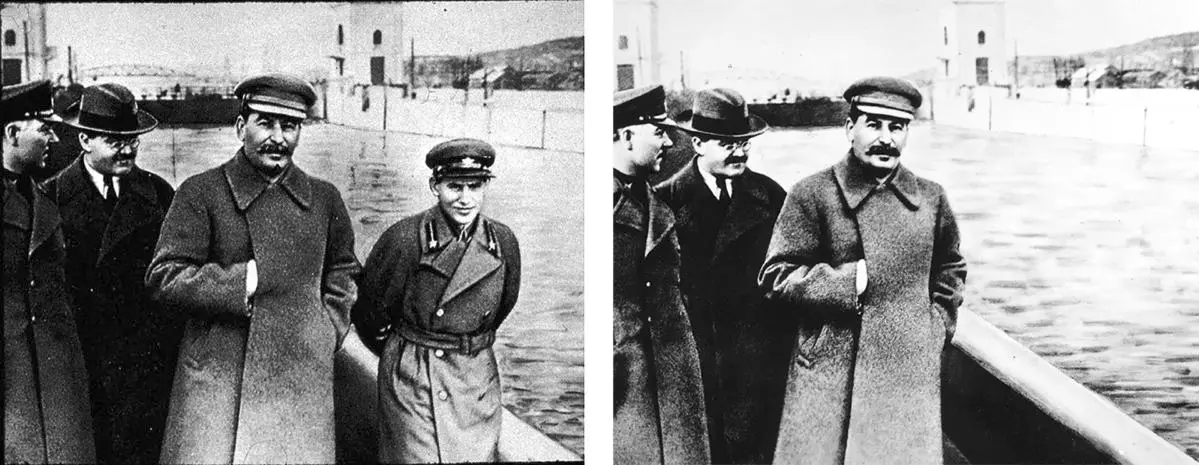
\includegraphics[width=0.5\linewidth]{dissertation//figures/stalin.png}
    \caption{A photo of Stalin and Yezhov which was subsequently edited to remove Yezhov}
    \label{fig:stalin-yezhov}
\end{figure}

With the advent of digital photography and computers, it photo manipulation became mainstream. Suddenly, images were not physical items but data stored on a computer which could be easily manipulated. Changes could be viewed instantly, reversed, and shared easily. Programs to edit images soon became possible such as Adobe Photoshop\footnote{\url{https://www.adobe.com/uk/products/photoshop.html}} and GIMP\footnote{\url{https://www.gimp.org/}}. Whilst these tools made photo editing cheap and accessible, they still required time, effort, and skill from humans in order to produce; an original image is also required for manipulation.

Computer Generated Imagery (CGI) is a technique primarily used in movies to add artificially augment a frame, often with complete novel additions. CGI was first used in the 1958 film ``Vertigo" and became widespread in the 1990s\cite{ozturk2023vicious}. In the present day, CGI is used in almost every blockbuster film to generate realistic images. In ``Rogue One: A Star Wars Story" the actor Peter Cushing digitally recreated after his death in 1994 to play Grand Moff Tarkin (Figure \ref{fig:tarkin}).While CGI requires large amounts of hardware, consumer image generation runs on much worse hardware but has equally progressed. Most modern social media apps contain a variety of beauty filters\cite{corcoran2014digital}. For example, a blur can be applied to reduce skin blemishes as shown by Figure \ref{fig:beauty-filter}. These are often less computationally expensive and so can run on smartphones, offering the ability to manipulate media to the masses, not just the technically-able and skilled.

\begin{figure}[H]
    \centering
    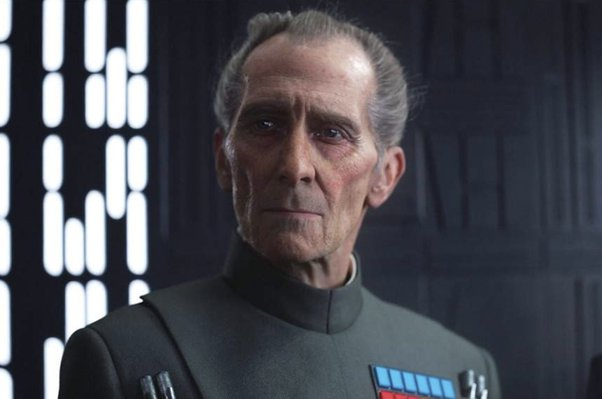
\includegraphics[width=0.5\linewidth]{dissertation//figures/grandmoff-tarkin.jpg}
    \caption{A digital recreation of Peter Cushing for the film ``Rogue One: A Star Wars Story"\cite{rogueone}}
    \label{fig:tarkin}
\end{figure}

\begin{figure}[H]
    \centering
    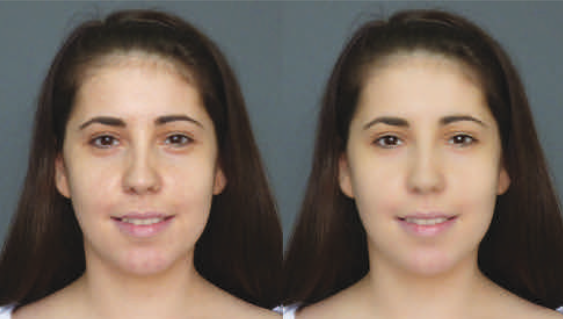
\includegraphics[width=0.5\linewidth]{dissertation//figures/blurring.png}
    \caption{An original image (left) blurred to remove skin blemishes (right)\cite{corcoran2014digital}}
    \label{fig:beauty-filter}
\end{figure}

\subsection{Artificial Intelligence for Manipulating Media}



\section{DeepFake Detection}

\subsection{Traditional Detection Methods}

\begin{itemize}
    \item Backbones
    \begin{itemize}
        \item ResNet, VGG19....
        \item Head added for final classification
        \item Often trained on imagenet (transfer learning)
    \end{itemize}
\end{itemize}

\subsection{Blink-Based Detection Methods}

\begin{itemize}
    \item Human's blink in a periodic and predictable manner
    \item DeepFakes struggle with temporal stuff
    \item Eye Aspect Ratio
    \item DeepVision
    \item Ictu Oculi
    \item see progress report for evaluation and other stuff
\end{itemize}

\section{Adversarial Noise}

\begin{itemize}
    \item Additive noise can cause misclassification
    \item Adversarial Perturbations
    \item FakeRetouch
    \item Again see progress report
\end{itemize}

\section{Datasets}

\begin{itemize}
    \item Wide variety of deepfake datasets (they be chonky)
    \item most require request for access
    \item DFDC is a pain
\end{itemize}